% !TeX program = xelatex 

\PassOptionsToPackage{prologue, dvipsnames}{xcolor}
\documentclass[AutoFakeBold,AutoFakeSlant]{beamer}
\usetheme{metropolis}           % Use metropolis theme
\setbeamercovered{transparent}
\usepackage{listings}
\usepackage{ThinctPPT}
 
% 支持中文的设置
\usepackage{xeCJK}
\usepackage{fontspec}
\setCJKmainfont[ItalicFont=思源宋体,BoldFont=SourceHanSerifSC-Bold]{Source Han Serif SC}
\newcommand{\KaiTi}{\CJKfontspec{楷体}}%用命令\fzkaiti调用方正楷体简体

% other packages
\usepackage{latexsym,amsmath,xcolor,multicol,booktabs,calligra}
\usepackage{graphicx,pstricks,listings,stackengine}

\title{Cookie崩溃分析报告}
\date{\today}
\author{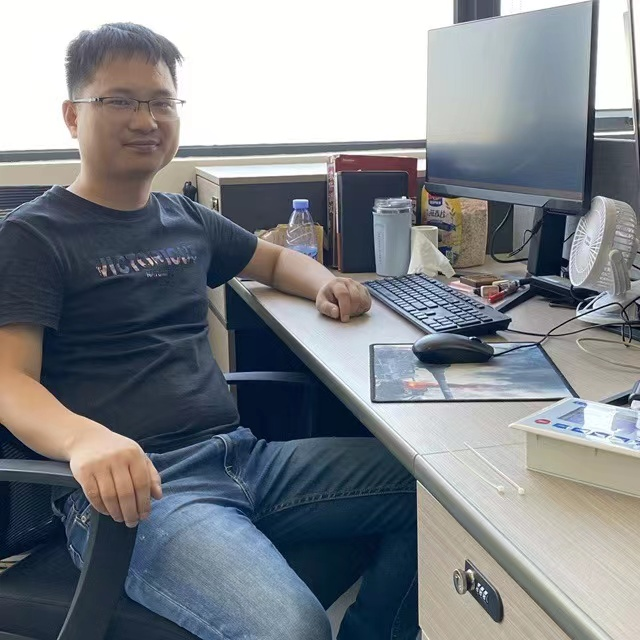
\includegraphics[width=0.26\linewidth]{ShowMe}\\THINCT}
\begin{document}
	\maketitle
	
	\section{构建崩溃现场}
	
	\begin{frame}[fragile]
		\LogoFrametitle{崩溃复现}
			\begin{figure}
			\centering % 将整个 figure 居中
			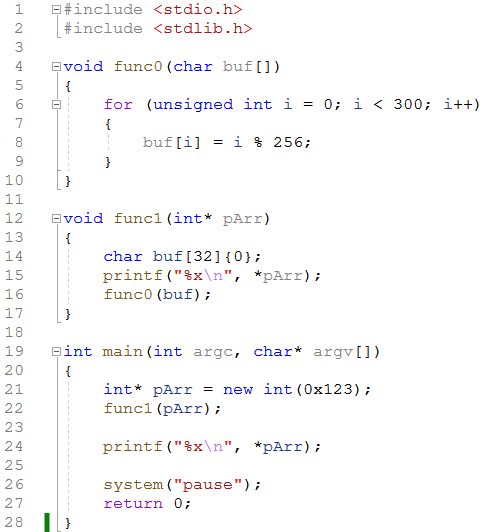
\includegraphics[width=0.6\linewidth]{1211srccode}
			\caption{源码构造浮现过程}
			\label{fig:sourcecode}
		\end{figure}
	\end{frame}
	
	\begin{frame} \LogoFrametitle{崩溃复现}
		\begin{figure}
			\centering % 将整个 figure 居中
			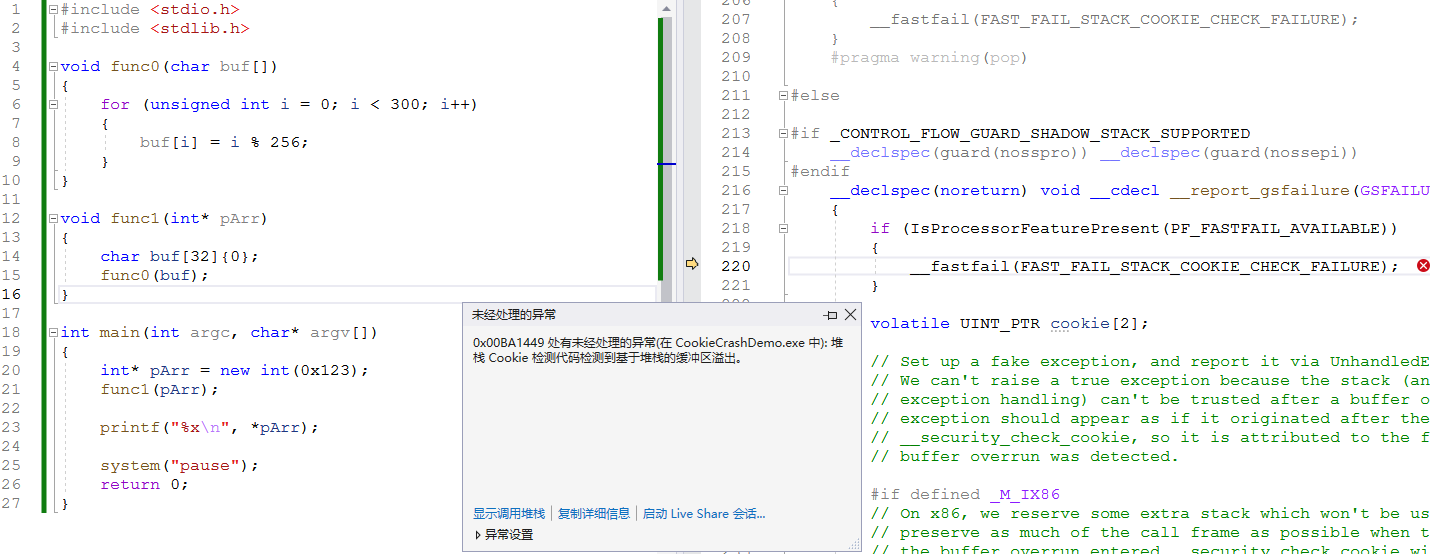
\includegraphics[width=1.6\linewidth]{1211crash}
			\caption{崩溃结果}
			\label{fig:crash show}
		\end{figure}
	\end{frame}
	
	\section{什么是cookie崩溃}
	\begin{frame}[fragile]
		\LogoFrametitle{cookie校验}
		\tiny
		堆栈(Stack)和堆(Heap)的 Cookie 安全检查是一种用于防止缓冲区溢出攻击的技术。这种技术的目的是通过引入一种额外的随机值(通常称为 Cookie)来增加攻击者预测攻击的难度,从而提高系统的安全性。
		
		堆栈 Cookie 安全检查:
		在堆栈 Cookie 安全检查中,通常是在函数的栈帧中添加一个随机生成的值,称为堆栈 Cookie 或 Canary。这个 Cookie 位于函数局部变量和返回地址之间,当函数返回时,会检查这个 Cookie 是否被破坏。
		
		攻击者如果试图通过溢出缓冲区来修改返回地址,他们也必须修改堆栈 Cookie。由于 Cookie 的值是不可预测的,攻击者需要事先知道这个 Cookie 的值才能成功执行攻击。因此,堆栈 Cookie 提供了一种防范缓冲区溢出攻击的机制。
		
		堆 Cookie 安全检查:
		堆 Cookie 安全检查与堆栈 Cookie 类似,但是是在动态内存分配的堆上进行的。在动态内存分配时,为分配的内存块添加了一个额外的 Cookie,并将这个 Cookie 存储在内存块的头部或尾部。当释放内存时,系统会检查 Cookie 是否被破坏,从而检测出潜在的堆溢出。
		
		实现原理:
		添加 Cookie:
		
		在函数调用或内存分配时,系统生成一个随机的 Cookie 值,并将其添加到相关数据结构中(堆栈帧或动态内存块)。
		检查 Cookie:
		
		在函数返回或内存释放时,系统会检查 Cookie 是否被破坏。如果 Cookie 被破坏,系统就会认为发生了缓冲区溢出,从而触发相应的安全措施。
		增加攻击者难度:
		
		由于 Cookie 是随机生成的,攻击者必须在进行攻击时预测正确的 Cookie 值,增加了攻击的难度。
		
	\end{frame}
	
	\begin{frame} \LogoFrametitle{cookie校验}
		\normalsize
		\begin{figure}
			\centering % 将整个 figure 居中
			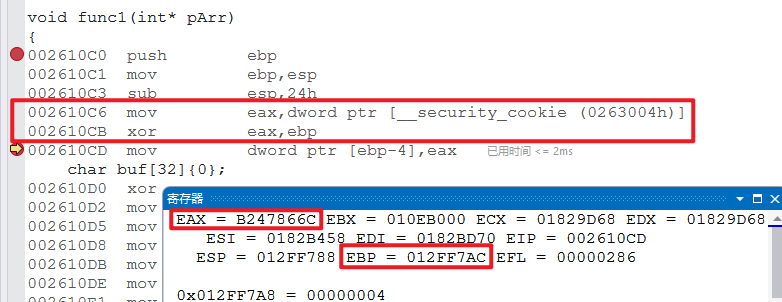
\includegraphics[width=\linewidth]{1211cookie01}
			\caption{cookie起点}
			\label{fig:cookie01}
		\end{figure}
	\end{frame}
	
	\begin{frame} \LogoFrametitle{cookie校验}
		\begin{figure}
			\centering % 将整个 figure 居中
			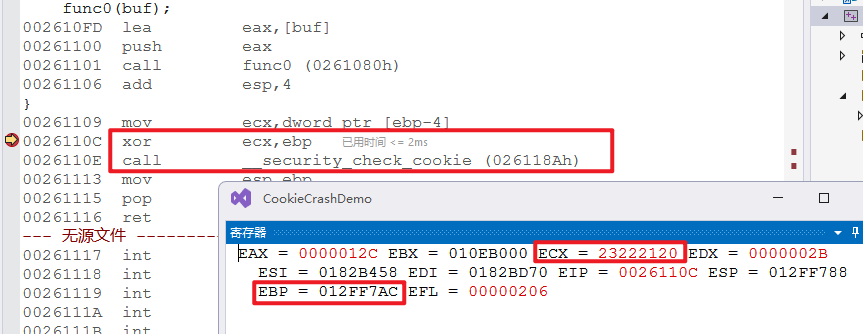
\includegraphics[width=\linewidth]{1211cookie02}
			\caption{cookie终点}
			\label{fig:cookie02}
		\end{figure}
	\end{frame}
	
	\begin{frame} \LogoFrametitle{cookie校验}
		\textbf{结论:}\\
		参与cookie相关的异或运算的两个值,ebp没有变化,另外eax和ecx在正常情况下应该是相同的,如果不相等,则说明堆栈出现破坏了.
	\end{frame}
		
	\section{分析方法}
	\begin{frame}[fragile]
		\LogoFrametitle{观察存放cookie抑或结果的内存}
		\begin{figure}
			\centering % 将整个 figure 居中
			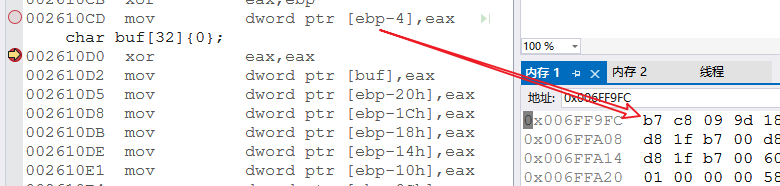
\includegraphics[width=\linewidth]{1211memwatch1}
			\caption{记住ebp-4所指向的内存的值}
			\label{fig:1211memwatch1}
		\end{figure}
	\end{frame}
	
	\begin{frame} \LogoFrametitle{观察存放cookie抑或结果的内存}
		\begin{figure}
			\centering % 将整个 figure 居中
			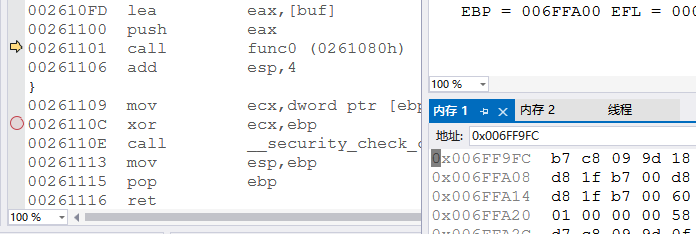
\includegraphics[width=\linewidth]{1211memwatch2}
			\caption{继续记住ebp-4所指向的内存的值}
			\label{fig:1211memwatch2}
		\end{figure}
	\end{frame}
	
	\begin{frame} \LogoFrametitle{观察存放cookie抑或结果的内存}
		\begin{figure}
			\centering % 将整个 figure 居中
			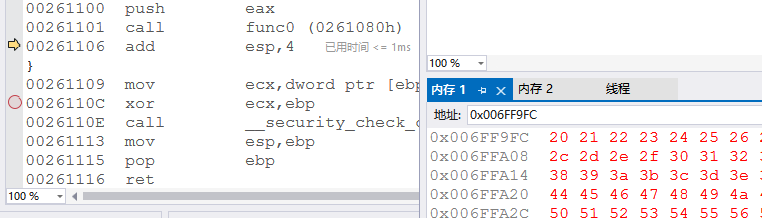
\includegraphics[width=\linewidth]{1211memwatch3}
			\caption{直到发生变化}
			\label{fig:1211memwatch2}
		\end{figure}
	\end{frame}
	
	\begin{frame} \LogoFrametitle{观察存放cookie抑或结果的内存}
		\textbf{总结:}\\
		只要这个哨兵位置的内存发生变化,就是发生了堆栈溢出.
	\end{frame}
		
	\section{思考}
	\begin{frame} \LogoFrametitle{你听懂了吗?}
		\textcolor{red}{\textbf{调试类似堆栈破坏的难点在哪里呢?}} 
	\end{frame}
	
\end{document}
